%%%% CAPÍTULO 2 - REVISÃO DA LITERATURA (OU REVISÃO BIBLIOGRÁFICA, ESTADO DA ARTE, ESTADO DO CONHECIMENTO)
%%
%% O autor deve registrar seu conhecimento sobre a literatura básica do assunto, discutindo e comentando a informação já publicada.
%% A revisão deve ser apresentada, preferencialmente, em ordem cronológica e por blocos de assunto, procurando mostrar a evolução do tema.
%% Título e rótulo de capítulo (rótulos não devem conter caracteres especiais, acentuados ou cedilha)
\chapter{Referencial te\'orico}\label{cap:referencialTeorico}

Neste capítulo, serão abordados diversos tópicos fundamentais relacionados ao processamento de imagens digitais. Inicialmente, serão apresentados conceitos essenciais sobre imagens digitais e suas propriedades (Seção 2.1), fornecendo uma base sólida para compreender os processos subsequentes. O processo de segmentação de imagens digitais e dados sintéticos será explorado nas Seções 2.1.1 a 2.1.5, oferecendo insights sobre técnicas e métodos empregados nesses domínios. Em seguida, a Seção 2.2 apresentará conceitos e modelos de Detecção de Objetos e técnicas relevantes relacionados ao tema. Por fim, será contextualizada a aplicação desses modelos na fusão de imagens e detecção de objetos na Seção 2.3 e subitens relacionados.

%Com o advento de técnicas avançadas como aprendizado de máquina e inteligência artificial, a capacidade de processar imagens com alta precisão tem se expandido significativamente. Redes Neurais Convolucionais (CNNs), por exemplo, têm revolucionado o campo do reconhecimento de imagens, fornecendo ferramentas poderosas para lidar com grandes conjuntos de dados de maneira eficaz (Krizhevsky et al., 2012).

\section{Processamento Digital de Imagens}\label{sec:fusao}



O \gls{pdi} representa um campo essencial dentro da Ciência da Computação, dedicado à manipulação e análise de imagens digitais através de algoritmos avançados. Conforme \citeonline{gonzalez2008digital} destacam, o objetivo primário do \gls{pdi} é extrair informações úteis, aprimorar a qualidade visual das imagens e tornar os dados mais acessíveis tanto para análises humanas quanto computacionais. Este processo envolve uma variedade de técnicas que incluem, mas não se limitam a, filtragem de ruído, segmentação de imagens, e detecção de bordas.

Além das aplicações tradicionais, como melhoramento de imagens médicas e reconhecimento de padrões, o \gls{pdi} tem visto uma expansão significativa de suas fronteiras devido ao advento da inteligência artificial e aprendizado profundo. As redes neurais convolucionais, por exemplo, têm revolucionado a forma como as imagens são processadas, permitindo avanços notáveis em tarefas como classificação de imagens e visão computacional aplicada à autonomia veicular \cite{Goodfellow2016,krizhevsky2012imagenet}.

\section{Fusão de Imagens}\label{sec:fusao}

A fusão de imagens é o processo de combinar várias imagens capturadas com perspectiva unificada, detectando áreas de sobreposição para alinhar e fundir as imagens com bordas imperceptíveis. As premissas incluem sobreposição suficiente, ausência de grandes movimentos e distorções mínimas nas imagens de entrada. O objetivo é produzir uma imagem panorâmica que se assemelhe à cena real, com emendas indetectáveis entre as imagens fundidas \cite{alomran2016feature}. Esse conceito é ilustrado na \autoref{fig:fusaoexemplo}.

\begin{figure}[H]%% Ambiente figure
    %\captionsetup{width=0.55\textwidth}%% Largura da legenda
    \caption{Fusão de quatro imagens para formar uma imagem panorâmica}%% Legenda
    \label{fig:fusaoexemplo}%% Rótulo
    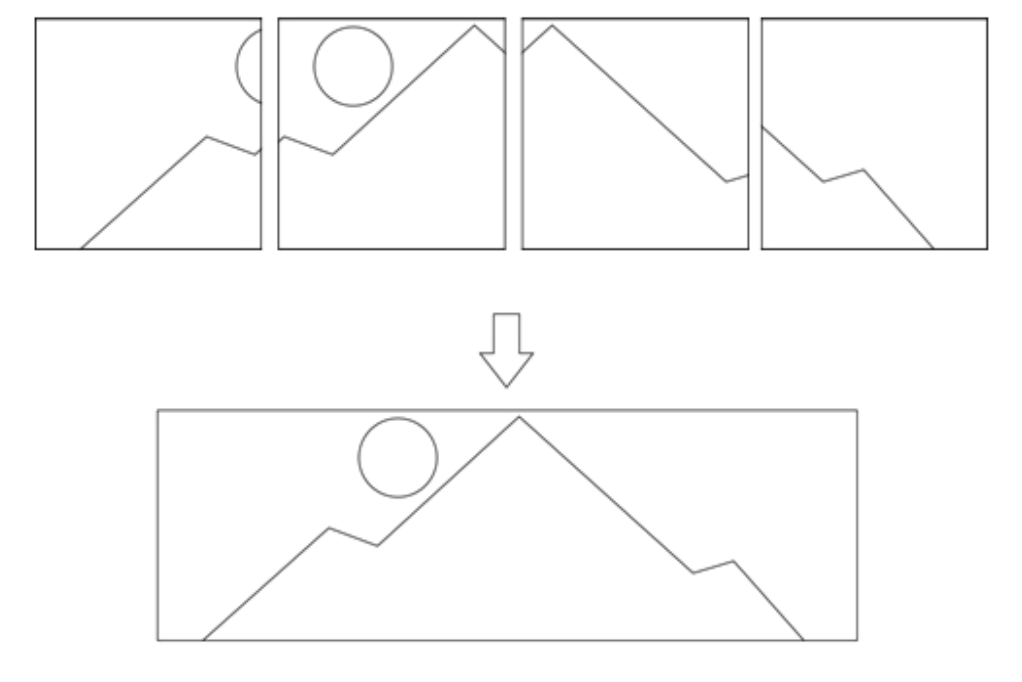
\includegraphics[scale=0.5]{figuras/fusao.png}%% Dimensões e localização
    \fonte{\citeonline{alomran2016feature}}%% Fonte
\end{figure}

A integração efetiva das imagens é realizada através de diversos métodos que podem ser categorizados em fusão baseada em pixel, fusão baseada em características e fusão a nível de decisão. Cada método tem suas próprias vantagens e é escolhido com base na especificidade da aplicação e na natureza das imagens a serem fundidas \cite{james2014multisensor}.

A fusão de imagens é amplamente aplicada em sensoriamento remoto, onde informações de várias imagens de satélite são combinadas para produzir uma representação mais detalhada da Terra. Em contextos médicos, a fusão é empregada para combinar imagens de diferentes modalidades, como Tomografia Computadorizada e Ressonância Magnética, para criar uma visão compreensiva das condições de saúde de um paciente, facilitando diagnósticos mais precisos e planejamento de tratamento eficaz \cite{li2017image,zhou2022medical}.

\subsection{Costura de Imagens (\textit{Image Stitching})}\label{subsec:sticthing}

O \textit{stitching} de imagens é um processo de Fusão de Imagem utilizado para combinar várias imagens com sobreposições parciais para criar uma imagem panorâmica contínua ou um mosaico. Esta técnica é fundamental em aplicações como a fotografia panorâmica, mapeamento e arte digital. Uma abordagem recente envolve o uso de algoritmos de aprendizado profundo para melhorar o alinhamento e a precisão das costuras, como mostrado por \citeonline{brown2020automatic}, que desenvolveram um método de detecção e correspondência de pontos de interesse que melhora significativamente a fluidez e a naturalidade das imagens resultantes, conforme exemplificado na \autoref{fig:stitching1}.

\begin{figure}[H]%% Ambiente figure
    %\captionsetup{width=0.55\textwidth}%% Largura da legenda
    \caption{Exemplo de fusão de imagens usando \textit{stitching}}%% Legenda
    \label{fig:stitching1}%% Rótulo
    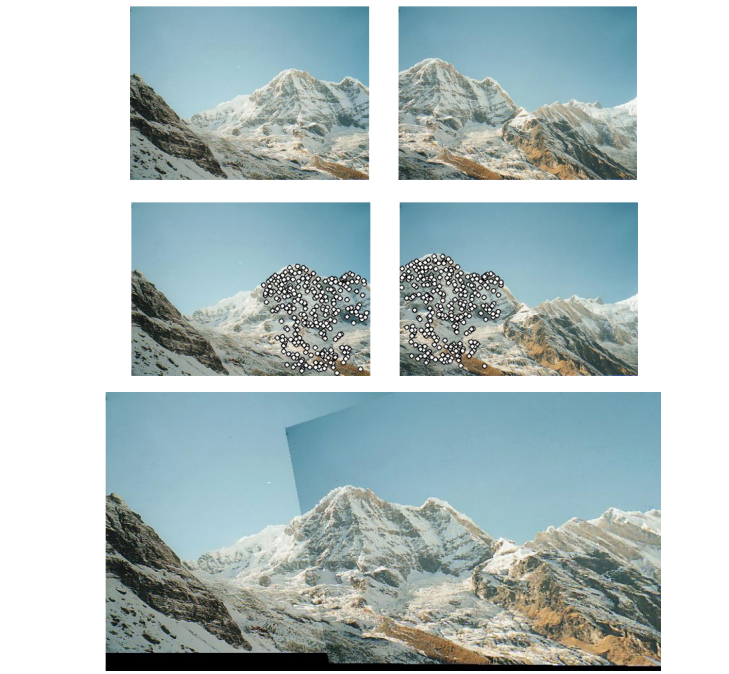
\includegraphics[scale=0.5]{figuras/referencialteorico/stitching1.png}%% Dimensões e localização
    \fonte{Adaptado de \citeonline{brown2020automatic}}%% Fonte
\end{figure}

A fusão de imagens por meio da técnica de \textit{stitching} é crucial para combinar múltiplas fotografias que possuem sobreposições parciais, criando uma única imagem panorâmica ou um mosaico detalhado. Esta abordagem é essencial em diversas aplicações práticas, como na fotografia panorâmica, que busca uma visão ampla de paisagens naturais ou urbanas, e no mapeamento geográfico, que exige composições detalhadas e abrangentes de uma área. De acordo com \citeonline{BrownLowe2007}, os avanços nas técnicas de aprendizado de máquina aplicadas ao \textit{stitching} de imagens têm resultado em melhorias significativas no alinhamento e na precisão das juntas, transformando a qualidade das composições panorâmicas. Eles afirmam:


\begin{citacao}
Desenvolvimentos recentes no aprendizado profundo possibilitaram técnicas mais sofisticadas de registro de imagens, que são críticas para alinhar imagens com precisão. Ao utilizar redes neurais convolucionais, agora podemos detectar e combinar características entre diferentes imagens com um alto grau de precisão, o que melhora significativamente a natureza contínua do panorama \cite{BrownLowe2007}.
\end{citacao}

Esta melhoria na tecnologia de detecção e correspondência de características é vital para o sucesso do \textit{stitching} de imagens, pois garante que as transições entre as imagens compostas sejam suaves e praticamente imperceptíveis, mantendo a integridade visual e a continuidade do panorama. Além disso, a aplicação de técnicas avançadas, como ajustes adaptativos de exposição e cor durante o processo, ajudam a resolver os desafios comuns relacionados à variação de iluminação entre as imagens originais, garantindo um resultado final mais homogêneo e visualmente agradável \cite{Szeliski2006}.

\subsection{Mesclagem de Imagens (\textit{Image Blending})}\label{subsec:blending}

A técnica de \textit{blending} ou mesclagem de imagens, é crucial no \gls{pdi}, onde a transição entre múltiplas imagens deve ser suave e imperceptível. Este processo é essencial tanto para aplicações práticas, como em fotografia panorâmica, quanto em contextos mais técnicos, como em realidade aumentada e visualizações médicas. As abordagens modernas para o \textit{blending} de imagens vão além dos métodos tradicionais, introduzindo técnicas avançadas que consideram a consistência de gradientes e a harmonização de cores para melhorar a qualidade visual das imagens compostas \cite{he2021adaptive}.

Um dos métodos mais influentes na área de mesclagem de imagens é descrito por \citeonline{Perez2003}, que propuseram a técnica de edição de imagens baseada em Poisson, um método que facilita a inserção de uma região de uma imagem em outra, preservando a consistência dos gradientes, o que é vital para uma transição suave entre as imagens. Esta técnica é particularmente útil para aplicações que requerem modificações na imagem sem que as junções se tornem visíveis, mantendo a integridade da iluminação e da textura originais ou removendo atributos desnecessários conforme indicado na \autoref{fig:fusao1}.

\begin{figure}
    \centering
    \caption{Ao aplicar uma fusão, é possível ocultar objetos completos, partes de objetos e artefatos indesejados de forma eficaz.}
    \label{fig:fusao1}
    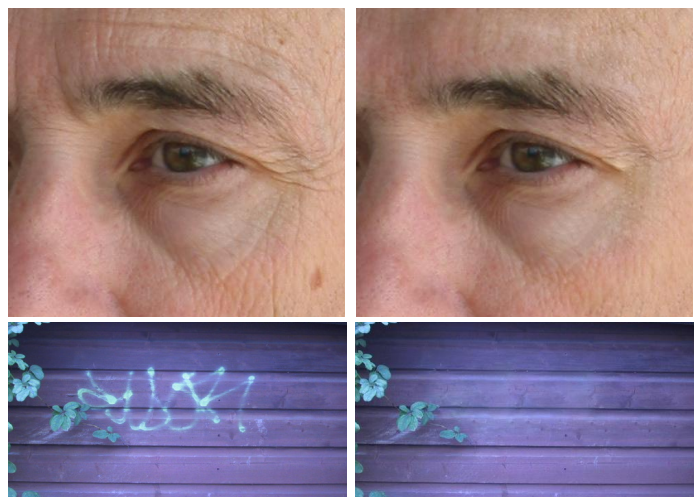
\includegraphics[width=0.5\linewidth]{figuras//referencialteorico/blending1.png}
\fonte{Adaptado de \citeonline{Perez2003}}%% Fonte

\end{figure}


Além disso, \citeonline{Farbman2009} introduziram uma abordagem baseada em mapeamento de coordenadas para \textit{blending} de texturas, que é extremamente eficaz na gestão de desafios relacionados com a variação de iluminação e textura entre as imagens a serem mescladas. Este método ajusta a textura das imagens para garantir que as características visuais sejam harmoniosas em toda a imagem composta, o que é crucial para aplicações em mapeamento geográfico e realidade virtual.

Também, a harmonização em múltiplas escalas, como explorado por \citeonline{Sunkavalli2010}, oferece uma solução sofisticada para o ajuste de imagens em várias escalas de detalhe. Esta técnica permite que as imagens compostas mantenham a consistência visual, ajustando características de alta e baixa frequência, o que é essencial para uma integração perfeita e para evitar discrepâncias visuais em panoramas ou em ambientes de realidade aumentada.

%\textit{Blending}, ou mesclagem de imagens, refere-se ao processo de combinar imagens de modo que a transição entre elas seja suave e imperceptível. Este método é frequentemente utilizado em conjunto com o \textit{stitching}, para suavizar as bordas onde as imagens se encontram. Técnicas avançadas de \textit{blending} utilizam métodos baseados em pixeis, como os apresentados por , que propõem um modelo de \textit{blending} adaptativo que ajusta os pesos de fusão com base nas características locais das imagens, resultando em uma transição mais suave e menos visível.e melhora significativamente a fluidez e a naturalidade das imagens resultantes.

\subsection{Fusão Multi-Exposição}\label{subsec:multiexposicao}


A técnica de fusão multi-exposição é um avanço significativo no campo do processamento de imagens, permitindo a combinação de várias imagens do mesmo cenário capturadas em diferentes configurações de exposição. Esta metodologia é essencial para capturar um maior dinamismo em cenas com variações extremas de luminosidade, garantindo que detalhes em áreas muito claras e muito escuras sejam preservados. \citeonline{zhang2020} desenvolveram um método inovador que emprega o conceito de \gls{cnn} para otimizar a seleção de características relevantes de cada exposição, o que resulta em uma imagem final com detalhes aprimorados e contraste superior \cite{zhang2020}. Este método representa um avanço considerável porque aborda diretamente o problema de perda de detalhes em áreas de alta ou baixa luminosidade, que é uma limitação comum em técnicas de fusão de imagens mais tradicionais.

Junto aos estudos de \citeonline{zhang2020}, outras pesquisas no campo têm contribuído para o desenvolvimento de técnicas ainda mais sofisticadas de fusão de imagens. Por exemplo, \citeonline{Mertens2007} propuseram uma abordagem que combina os melhores \textit{pixels} de uma série de imagens com diferentes exposições usando uma estratégia de decomposição em pirâmide de \textit{Laplace}, o que permite uma transição suave entre as áreas de diferentes exposições dentro da imagem composta \cite{Mertens2007}. Essa técnica é particularmente útil em fotografia \gls{hdr}, onde é crucial manter uma representação natural do ambiente sem sacrificar os detalhes visuais.

Por fim, o potencial das técnicas de fusão multi-exposição para aplicações práticas é vasto, estendendo-se além da fotografia para áreas como videografia e vigilância, onde condições de iluminação variáveis podem afetar significativamente a qualidade das imagens capturadas. \citeonline{Goshtasby2007} exploraram o uso de algoritmos de alinhamento e fusão em imagens de vídeo, mostrando como a fusão multi-exposição pode ser adaptada para melhorar a qualidade de vídeos em tempo real, oferecendo um método robusto para otimizar a visibilidade em diversas condições de iluminação \cite{Goshtasby2007}. Essas pesquisas ilustram como a fusão de imagens se adapta continuamente para atender às exigências de novas aplicações e tecnologias, tornando-a um campo de estudo fundamental na ciência da computação e processamento de imagens.

%A fusão multi-exposição é usada para combinar imagens do mesmo cenário tiradas com diferentes configurações de exposição para capturar detalhes em áreas muito claras ou muito escuras. \citeonline{zhang2020} introduziram um método de fusão multi-exposição que utiliza CNNs para otimizar a seleção de características relevantes de cada exposição, maximizando assim a qualidade da imagem final em termos de detalhes e contraste.

 \subsection{Fusão Multi-Focal}\label{subsec:multifocal}

%Em cenários onde objetos em diferentes profundidades precisam ser claramente visualizados, a fusão multi-focal combina várias imagens focadas em diferentes distâncias para criar uma imagem única com todos os objetos em foco. \citeonline{li2021multifocal} desenvolveram uma técnica que utiliza análise de frequência espacial para determinar as áreas de foco em cada imagem e combiná-las de forma eficiente.

A fusão multi-focal é uma técnica avançada no processamento de imagens que atende às necessidades de visualizar claramente objetos em várias profundidades dentro de uma única imagem. Esta abordagem é extremamente útil em campos como a microscopia e a fotografia macro, onde a profundidade de campo limitada pode ser um obstáculo significativo. \citeonline{Tian2020} introduziram uma inovação notável nesta área ao desenvolver uma técnica que emprega redes neurais convolucionais para identificar eficientemente as áreas de foco em múltiplas imagens capturadas em diferentes distâncias focais. Ao combinar estas imagens focadas de forma seletiva, essa técnica permite a criação de uma imagem composta em que todos os elementos são exibidos em foco, otimizando a visualização detalhada de toda a cena.

Além do trabalho de \citeonline{Tian2020}, \citeonline{li2021multifocal} contribuíram significativamente para a área de fusão multi-focal com sua pesquisa sobre fusão de imagens usando filtragem guiada. Esta abordagem não só melhora a qualidade da fusão por meio de técnicas avançadas de processamento de imagem, mas também assegura a integridade dos detalhes e a consistência das cores nas imagens finais. Sua metodologia oferece uma solução robusta para superar as limitações das abordagens tradicionais, proporcionando resultados que são tanto visualmente impressionantes quanto tecnicamente precisos \cite{li2021multifocal}.

A relevância da fusão multi-focal se estende para além de sua aplicação em fotografia e microscopia, tendo implicações significativas também em campos como vigilância e segurança. \citeonline{Ma2021} exploraram o uso de técnicas de transferência de gradiente e minimização da variação total para a fusão de imagens infravermelhas e visíveis. Este método melhora notavelmente a visibilidade em condições de iluminação adversas, permitindo uma melhor detecção e identificação em sistemas de vigilância, onde diferentes modalidades de imagem precisam ser combinadas para uma interpretação eficaz.

 \subsection{Fusão \textit{Wavelet}}\label{subsec:wavelet}
 A transformada \textit{wavelet} é amplamente reconhecida por sua eficácia no processamento de imagens, particularmente na fusão de imagens, devido à sua habilidade de decompor imagens em múltiplos níveis de resolução. Essa técnica permite analisar as imagens em diferentes escalas, capturando eficientemente as características locais e globais. Segundo \citeonline{mallat2009wavelet}, a transformada \textit{wavelet} separa os componentes de frequência das imagens em coeficientes de baixa e alta frequência, que correspondem, respectivamente, às características de aproximação e detalhes das imagens.

No processo de fusão usando transformada \textit{wavelet}, cada imagem de entrada é decomposta em vários níveis de detalhes por meio da transformada. Após essa decomposição, os coeficientes de aproximação e detalhes de diferentes imagens são combinados seguindo regras específicas de fusão. Este método foi aprimorado por \citeonline{lewis2020adaptive}, que desenvolveram uma abordagem adaptativa para a seleção de coeficientes, visando maximizar a transferência de informação relevante para a imagem final, resultando em uma reconstrução mais precisa e com maior integridade visual.

A fusão de imagens usando a transformada \textit{wavelet} envolve a decomposição de cada imagem em múltiplos níveis de resolução, seguida pela combinação dos coeficientes para formar a imagem final, de acordo com as equações demonstradas:
\begin{itemize}
    \item \textbf{Decomposição \textit{Wavelet}}:
    Cada imagem \( I \) é decomposta em coeficientes de aproximação \( A \) e detalhes \( D \) usando a transformada \textit{wavelet}, apresentada na 
Equação\ref{eq:decomposicao}:

\begin{equation}
W(I) = (A, D)
\label{eq:decomposicao}
\end{equation}
\end{itemize}

\begin{itemize}
\item{\textbf{Combinação de Coeficientes}}
Os coeficientes de aproximação e detalhes de diferentes imagens são combinados usando regras específicas de fusão, conforme mostrado na Equação \ref{eq:combinacao}:

\begin{equation}
F = \text{Fusão}(A_1, A_2, \ldots; D_1, D_2, \ldots)
\label{eq:combinacao}
\end{equation}

\end{itemize}

\begin{itemize}
\item{\textbf{Reconstrução da Imagem}}
A imagem final é reconstruída a partir dos coeficientes fusionados, conforme representado na Equação \ref{eq:reconstrucao}:
\begin{equation}
   I_{\text{final}} = W^{-1}(F)
   \label{eq:reconstrucao}
\end{equation}

\end{itemize}

Na Equação \ref{eq:reconstrucao}, \( \text{I}_{\text{final}} \) representa a imagem final reconstruída, que é obtida aplicando a transformada inversa de \textit{wavelet} (\( W^{-1} \)) sobre os coeficientes fusionados (\( F \)). O processo começa com a aplicação da transformada \textit{wavelet} às imagens originais, decompondo-as em diferentes níveis de resolução e gerando coeficientes que capturam tanto detalhes finos quanto aproximações globais. Esses coeficientes são então combinados usando uma estratégia de fusão específica, resultando em um conjunto de coeficientes fusionados (\( F \)) que mantém as características desejadas de cada imagem original. A transformada inversa de \textit{wavelet} (\( W^{-1} \)) é então aplicada a esses coeficientes fusionados para reconstruir a imagem final no domínio espacial. 

A fusão \textit{wavelet} é particularmente vantajosa devido à sua capacidade de manter a integridade das informações espaciais e de resolução das imagens originais, ao mesmo tempo que minimiza a perda de informação e artefatos de ruído. Uma inovação recente nessa área foi introduzida por \citeonline{zhang2021}, que propuseram um novo algoritmo baseado em \textit{wavelet} para a fusão de imagens médicas, que melhora significativamente a clareza e o contraste das imagens resultantes, crucial para aplicações em diagnósticos médicos precisos.

\section{Mosaico de Imagens}\label{sec:mosaico}

O mosaico de imagens é uma técnica consolidada na visão computacional que permite a fusão de múltiplas imagens para formar uma única composição detalhada. Este processo não é apenas uma questão de sobreposição, mas envolve um alinhamento preciso e uma fusão meticulosa para garantir a continuidade visual sem falhas perceptíveis. Segundo \citeonline{Szeliski2010}, a técnica de mosaico de imagens é essencial para criar uma visão panorâmica ampla a partir de imagens parciais estreitas, o que é crítico em aplicações como a imagem médica e a fotografia aérea.

%Recentemente, as Redes Neurais Convolucionais (CNNs) têm sido aplicadas com sucesso no mosaico de imagens, oferecendo uma abordagem mais robusta e eficaz, reduzindo a dependência de características superficiais e melhorando a qualidade do resultado final \cite{Shi2020}.  Além disso, métodos de blending para mosaico de imagens desempenham um papel crucial na suavização de transições e na preservação de bordas nítidas, sendo categorizados em diferentes abordagens, como suavização de transições, domínio de gradientes e costura ótima \cite{GHOSH20161}.

As aplicações dos mosaicos de imagens são tão variadas quanto suas técnicas. Na medicina, por exemplo, o mosaico de imagens permite aos médicos visualizar uma região extensa de tecido em detalhes microscópicos, o que é fundamental para diagnósticos precisos e planejamento de tratamento \cite{Zitova2003}. Na robótica, veículos autônomos utilizam mosaicos de imagens para uma compreensão abrangente do ambiente, facilitando a navegação e a tomada de decisões autônomas \cite{Scaramuzza2011}.

\subsection{Algoritmos de Mosaico de Imagens}\label{sec:algoritmosmosaico}

No contexto técnico, a criação de um mosaico envolve várias etapas complexas, incluindo a detecção de características, a correspondência de pontos de interesse entre imagens, e a aplicação de transformações geométricas para alinhar as imagens \cite{BrownLowe2007}. Esses autores destacam que o sucesso do mosaico de imagens depende crucialmente da precisão na correspondência de características, que pode ser desafiada por fatores como iluminação variável e mudanças de perspectiva entre as imagens.

Métodos de mosaico de imagens são cruciais para a criação de imagens panorâmicas ou esticadas. O Algoritmo de Cantos de Harris é amplamente utilizado devido à sua robustez e invariância à rotação, embora seja sensível à escala. Por outro lado, o Algoritmo \gls{fast} é vantajoso por ser invariante tanto à rotação quanto à escala, com um tempo de execução otimizado, apesar de apresentar desempenho reduzido na presença de ruído. Enquanto isso, o Algoritmo SIFT se destaca pela sua invariância tanto à rotação quanto à escala, bem como pela eficácia na presença de ruído, embora seja suscetível a variações na iluminação \cite{vaghela2014review}. Esses conceitos serão abordados de forma mais completa a seguir.

\subsection{Mosaico Panorâmico de Visão Completa}\label{sec:mosaicocompleto}

Mosaico panorâmico de visão completa é uma técnica utilizada para criar imagens panorâmicas contínuas que abrangem um amplo campo de visão. Uma abordagem comum para criar mosaicos panorâmicos envolve a costura de múltiplas imagens parciais capturadas de diferentes pontos de vista em uma cena. Isso geralmente é realizado por meio da identificação de pontos de correspondência entre as imagens parciais e a aplicação de técnicas de registro e transformação para alinhar e combinar as imagens de forma que elas se sobreponham perfeitamente. A abordagem para costurar imagens livres é uma variante desse processo que permite a criação de mosaicos panorâmicos a partir de imagens capturadas livremente, sem a necessidade de movimentos controlados ou restrições específicas de captura. Essa abordagem oferece maior flexibilidade e liberdade na captura de imagens panorâmicas, permitindo a criação de mosaicos de alta qualidade em uma variedade de cenários e condições de captura \cite{Szeliski2006}.

\subsection{Algoritmo de Cantos de \textit{Harris}}\label{}

O Algoritmo de Cantos de \textit{Harris} é uma técnica clássica de detecção de cantos em imagens. Proposto por \citeonline{harris1988combined}, este algoritmo identifica regiões na imagem onde há mudanças significativas de intensidade em todas as direções. Ele calcula a matriz de autovalores da função de covariância dos gradientes locais da imagem e usa esses autovalores para determinar a presença de cantos. Abaixo seguem as formulações matemáticas que descrevem esse conceito:

A função de energia \( E \) para um deslocamento \( (\Delta x, \Delta y) \) é descrita na Equação \ref{eq:harris1}, onde \( w(x, y) \) é uma função de janela que pondera os \textit{pixels} próximos ao centro \( (x, y) \).

\begin{equation}
    E(\Delta x, \Delta y) = \sum_{x,y} w(x, y) \left[I(x + \Delta x, y + \Delta y) - I(x, y)\right]^2
    \label{eq:harris1}
\end{equation}


A matriz de segundo momento \( M \) é representada abaixo na Equação \ref{eq:harris2}.

\begin{equation}
    M = \sum_{x,y} w(x, y) \begin{bmatrix} I_x^2 & I_x I_y \\ I_x I_y & I_y^2 \end{bmatrix}
    \label{eq:harris2}
\end{equation}


Por fim, a resposta característica \( R \) é calculada com a Equação \ref{eq:harris3}.

\begin{equation}
   R = \det(M) - k \cdot (\text{trace}(M))^2
   \label{eq:harris3}
\end{equation}


Os cantos são pontos onde os autovalores são grandes em magnitude e aproximadamente iguais, indicando que a mudança de intensidade é significativa em todas as direções. Embora o Algoritmo de Cantos de \textit{Harris} seja robusto e invariante à rotação, ele pode não funcionar bem em escalas diferentes e pode ser sensível a ruídos \cite{vaghela2014review}.


\subsection*{Otimização com Verificação Acelerada}

Para otimizar o processo de detecção, inicialmente apenas 4 \textit{pixels} são testados. Se nenhum deles atender ao critério, o \textit{pixel} \( p \) é rapidamente descartado como um canto potencial.

\[
\text{Se} \, (I_1 > I_p + t) \, \text{e} \, (I_9 > I_p + t) \, \text{e} \, (I_5 > I_p + t) \, \text{e} \, (I_{13} > I_p + t) \, \text{então} \, p \, \text{é um canto}
\]

Ele usa um teste simples e eficiente para determinar se um \textit{pixel} é um canto ou não, comparando as intensidades de \textit{pixels} em torno de um círculo com o \textit{pixel} central. O Algoritmo \gls{fast} é vantajoso por sua rapidez de execução e invariância à rotação, mas pode apresentar desempenho fraco na presença de ruído \cite{vaghela2014review}.

\subsection{Algoritmo \gls{sift}}\label{}

O Algoritmo \gls{sift} é uma técnica amplamente utilizada para detectar e descrever características em imagens. Proposto por \citeonline{lowe99}, o \gls{sift} identifica pontos de interesse que são invariantes à escala, rotação e iluminação. Ele extrai descritores locais robustos em torno desses pontos de interesse, que são usados para realizar correspondência entre diferentes imagens.

O \gls{sift} é conhecido por sua eficácia na presença de transformações geométricas e variações de iluminação, tornando-o uma escolha popular em aplicações de reconhecimento de objetos e mapeamento 3D \cite{vaghela2014review}. Ele detecta e descreve características locais em imagens, sendo invariante a mudanças de escala, rotação e iluminação. As etapas principais incluem:

\subsection*{Geração do Espaço-Escala}
A imagem é convolvida com filtros Gaussianos de várias escalas, conforme a Equação \ref{eq:espacoescala}:
\begin{equation}
    L(x, y, \sigma) = G(x, y, \sigma) \ast I(x, y)
    \label{eq:espacoescala}
\end{equation}

Nesta equação, \(L(x, y, \sigma)\) representa a imagem suavizada em um ponto \((x, y)\) com uma escala \(\sigma\). A função \(G(x, y, \sigma)\) é a função Gaussiana com desvio padrão \(\sigma\), usada para suavizar a imagem. A imagem original é representada por \(I(x, y)\), e \(\ast\) denota a operação de convolução.

A Diferença de Gaussianas, do inglês \gls{dog}, é calculada na Equação \ref{eq:dog}:
\begin{equation}
    D(x, y, \sigma) = L(x, y, k\sigma) - L(x, y, \sigma)
    \label{eq:dog}
\end{equation}

Aqui, \(D(x, y, \sigma)\) representa a diferença entre duas imagens suavizadas em escalas \(\sigma\) e \(k\sigma\). O parâmetro \(k\) é uma constante multiplicativa que define a escala relativa entre duas imagens suavizadas.

\subsection*{Localização de Pontos-Chave}
Pontos extremos são identificados na pirâmide \gls{dog}. Os candidatos a pontos-chave são refinados usando a Equação \ref{eq:pc}:

\begin{equation}
    D(\mathbf{x}) = D + \frac{\partial D}{\partial \mathbf{x}}^T \mathbf{x} + \frac{1}{2} \mathbf{x}^T \frac{\partial^2 D}{\partial \mathbf{x}^2} \mathbf{x}
    \label{eq:pc}
\end{equation}


Nesta equação, \(D\) é o valor da \gls{dog} no ponto-chave candidato, e \(\mathbf{x}\) é o vetor de posição \((x, y, \sigma)\) do ponto-chave. O termo \(\frac{\partial D}{\partial \mathbf{x}}\) representa o gradiente da \gls{dog} em relação a \(\mathbf{x}\), enquanto \(\frac{\partial^2 D}{\partial \mathbf{x}^2}\) é a Hessiana da \gls{dog} em relação a \(\mathbf{x}\).

\subsection*{Atribuição de Orientação}
Cada ponto-chave recebe uma orientação baseada nos gradientes locais, de acordo com a Equação \ref{eq:pc2}:

\begin{equation}
\theta(x, y) = \tan^{-1}\left(\frac{L_y}{L_x}\right)
    \label{eq:pc2}
\end{equation}

Aqui, \(\theta(x, y)\) é a orientação do ponto-chave no ponto \((x, y)\). Os termos \(L_x\) e \(L_y\) representam os gradientes da imagem suavizada nas direções \(x\) e \(y\), respectivamente.

\subsection*{Criação do Descritor de Pontos-Chave}
Os descritores são formados por vetores de características locais, garantindo robustez, conforme ilustrado na Equação \ref{eq:descritor}:

\begin{equation}
    \text{Descritor} = \left[\text{Gradientes locais de magnitude e orientação}\right]
    \label{eq:descritor}
\end{equation}

O descritor é um vetor que descreve a vizinhança local do ponto-chave, incluindo informações sobre os gradientes de magnitude e orientação.

Estas etapas tornam o \gls{sift} eficaz para aplicações de visão computacional que exigem detecção e correspondência precisas de características em diferentes condições de imagem.

% Simplified comments for each variable
% - \(L(x, y, \sigma)\): Smoothed image at point (x, y) with scale \(\sigma\).
% - \(G(x, y, \sigma)\): Gaussian function with standard deviation \(\sigma\), used to smooth the image.
% - \(I(x, y)\): Original image.
% - \(\ast\): Convolution operation.
% - \(D(x, y, \sigma)\): Difference of Gaussians (DoG) at point (x, y) with scale \(\sigma\).
% - \(k\): Constant factor for scale.
% - \(D\): Value of DoG at the candidate keypoint.
% - \(\mathbf{x}\): Position vector (x, y, \(\sigma\)) of the keypoint.
% - \(\frac{\partial D}{\partial \mathbf{x}}\): Gradient of DoG with respect to \(\mathbf{x}\).
% - \(\frac{\partial^2 D}{\partial \mathbf{x}^2}\): Hessian of DoG with respect to \(\mathbf{x}\).
% - \(\theta(x, y)\): Orientation of the keypoint at point (x, y).
% - \(L_x\): Gradient of the smoothed image in the x direction.
% - \(L_y\): Gradient of the smoothed image in the y direction.
% - Descritor: Vector describing the local neighborhood of the keypoint, including magnitude and orientation gradients.



\subsection{Fusão Híbrida de Imagens}\label{}

A fusão híbrida de imagens tem se destacado como uma abordagem promissora para melhorar o desempenho em tarefas de visão computacional. Abordagens como \textit{Mixup}, \gls{ganmdb} e estratégias baseadas em políticas de otimização têm demonstrado resultados impressionantes, aumentando a precisão e superando outras técnicas em diferentes conjuntos de dados de referência \cite{XU2023109347}. O \textit{Mixup}, por exemplo, tem sido eficaz na melhoria da precisão de classificação em conjuntos de dados como \textit{ImageNet-2012\footnote{https://image-net.org/index.php}}, enquanto o \gls{ganmdb} tem alcançado resultados notáveis na classificação de imagens, especialmente em conjuntos de dados desafiadores como \textit{102Flowers\footnote{https://www.robots.ox.ac.uk/~vgg/data/flowers/102/}} \cite{XU2023109347}. 

Além disso, estratégias baseadas em políticas de otimização têm sido exploradas para melhorar ainda mais o desempenho e a eficiência de algoritmos de fusão de imagens, destacando a importância contínua do desenvolvimento e aplicação de técnicas avançadas nessa área em constante evolução \cite{XU2023109347}.

\begin{itemize}
    \item \textbf{Abordagens como \textit{Mixup}:} Abordagens como \textit{Mixup} têm ganhado destaque recentemente como uma técnica eficaz para aumentar a generalização e melhorar o desempenho de modelos de aprendizado de máquina. \textit{Mixup} é uma técnica de aumento de dados que combina pares de exemplos de treinamento para criar novos exemplos, interpolando linearmente entre as características e os rótulos desses exemplos. Essa abordagem ajuda a suavizar a superfície de decisão do modelo, tornando-o mais robusto a variações nos dados de entrada e reduzindo o risco de \textit{overfitting}. \textit{Mixup} tem sido amplamente utilizado em tarefas de classificação de imagens, alcançando melhorias significativas na precisão e na capacidade de generalização dos modelos \cite{zhang2017mixup}.
    \item \textbf{GAN-MDB: }\gls{ganmdb} é uma abordagem baseada em redes generativas adversariais, do inglês,  \gls{gan}, para realizar tarefas de predição densa e multi-ramificada em imagens. \gls{ganmdb} usa uma arquitetura de rede neural que consiste em um gerador e um discriminador, onde o gerador produz múltiplas saídas densas e ramificadas, e o discriminador avalia a qualidade dessas saídas em relação aos rótulos reais. Essa abordagem permite a geração de predições detalhadas e de alta resolução, melhorando o desempenho em tarefas como segmentação semântica e detecção de objetos em imagens \cite{fan2019ganmbd}.
    \item Estratégias baseadas em políticas de otimização: Estratégias baseadas em políticas de otimização têm sido amplamente exploradas para melhorar o desempenho e a eficiência de algoritmos de fusão de imagens. Essas estratégias envolvem o ajuste de parâmetros e hiper parâmetros do modelo com base em uma política de otimização específica, como algoritmos genéticos, algoritmos evolutivos ou otimização baseada em gradiente. Ao adaptar automaticamente os parâmetros do modelo durante o treinamento, essas estratégias permitem uma exploração mais eficiente do espaço de busca e uma convergência mais rápida para soluções de alta qualidade. Estratégias baseadas em políticas de otimização têm sido aplicadas com sucesso em uma variedade de tarefas de visão computacional, incluindo fusão de imagens, detecção de objetos e segmentação de imagens \cite{pmlr-v119-tian20a}.
\end{itemize}


%% tag-novo

\section{Métricas de Avaliação}

A avaliação adequada de sistemas de fusão de imagens e detecção de objetos requer o uso de métricas quantitativas e qualitativas que permitam mensurar o desempenho das técnicas implementadas. Esta seção apresenta as principais métricas utilizadas tanto para avaliar a qualidade da fusão de imagens quanto para mensurar a eficácia da detecção de objetos.

\subsection{Métricas para Fusão de Imagens}

A qualidade das imagens panorâmicas geradas por meio de técnicas de fusão pode ser avaliada através de diversas métricas objetivas que quantificam aspectos como preservação de informação, qualidade visual e eficiência computacional.

%% alterado-20250127-metricas
\subsubsection{Peak Signal-to-Noise Ratio (PSNR)}

O PSNR (\textit{Peak Signal-to-Noise Ratio}) é uma das métricas mais amplamente utilizadas para avaliar a qualidade de imagens processadas, medindo a relação entre o sinal máximo possível e o ruído introduzido durante o processamento. Esta métrica quantifica objetivamente a degradação da qualidade da imagem em termos de erro quadrático médio. Segundo \cite{wang2004image}, o PSNR é calculado conforme a Equação~\ref{eq:psnr}:

\begin{equation}
\label{eq:psnr}
PSNR = 10 \cdot \log_{10}\left(\frac{MAX^2_I}{MSE}\right)
\end{equation}

\noindent onde $MAX_I$ representa o valor máximo possível de pixel na imagem (tipicamente 255 para imagens de 8 bits) e $MSE$ (\textit{Mean Squared Error}) é o erro quadrático médio entre a imagem de referência e a imagem processada, calculado pela Equação~\ref{eq:mse}:

\begin{equation}
\label{eq:mse}
MSE = \frac{1}{mn} \sum_{i=1}^{m}\sum_{j=1}^{n}[I(i,j) - K(i,j)]^2
\end{equation}

Nesta equação, $m$ e $n$ são as dimensões da imagem, $I(i,j)$ representa a imagem de referência e $K(i,j)$ a imagem fusionada. O PSNR é expresso em decibéis (dB) e valores mais altos indicam menor ruído e melhor qualidade da imagem processada. Na prática, valores acima de 30 dB são geralmente considerados aceitáveis para aplicações de fusão de imagens, valores entre 30-40 dB indicam boa qualidade, e valores acima de 40 dB representam qualidade excelente com ruído praticamente imperceptível \cite{hore2010image}.

Uma limitação importante do PSNR é que, apesar de ser uma métrica objetiva e amplamente utilizada, nem sempre corresponde perfeitamente à percepção visual humana. Duas imagens com o mesmo valor de PSNR podem ser percebidas de forma diferente por observadores humanos, especialmente quando os tipos de distorção são distintos. Por essa razão, o PSNR é frequentemente utilizado em conjunto com outras métricas, como o SSIM, para uma avaliação mais completa da qualidade da fusão de imagens \cite{hore2010image}.
%% alterado-20250127-metricas

%% alterado-20250127-metricas
\subsubsection{Structural Similarity Index (SSIM)}

O índice SSIM (\textit{Structural Similarity Index}) foi desenvolvido para superar algumas limitações do PSNR, fornecendo uma avaliação mais consistente com a percepção visual humana. Diferentemente do PSNR, que trata qualquer distorção como ruído, o SSIM analisa mudanças estruturais na imagem, considerando como o sistema visual humano realmente percebe qualidade. \cite{wang2004image} propuseram esta métrica que considera três componentes fundamentais: luminância, contraste e estrutura. O SSIM é calculado conforme a Equação~\ref{eq:ssim}:

\begin{equation}
\label{eq:ssim}
SSIM(x,y) = \frac{(2\mu_x\mu_y + C_1)(2\sigma_{xy} + C_2)}{(\mu^2_x + \mu^2_y + C_1)(\sigma^2_x + \sigma^2_y + C_2)}
\end{equation}

\noindent onde $\mu_x$ e $\mu_y$ são as médias locais das imagens $x$ e $y$ (componente de luminância), $\sigma^2_x$ e $\sigma^2_y$ são as variâncias (componente de contraste), $\sigma_{xy}$ é a covariância (componente de estrutura), e $C_1$ e $C_2$ são constantes pequenas para estabilizar a divisão quando os denominadores são próximos de zero.

Teoricamente, o SSIM varia entre -1 e 1, onde 1 indica similaridade perfeita entre as imagens. Na prática, ao comparar imagens naturais processadas, os valores tipicamente ficam no intervalo de 0 a 1, sendo que valores acima de 0,90 indicam qualidade excelente, valores entre 0,80-0,90 indicam boa qualidade, e valores abaixo de 0,80 sugerem degradação perceptível na qualidade da imagem \cite{wang2004image}. Valores negativos são teoricamente possíveis mas raramente observados em aplicações práticas de fusão de imagens.

Esta métrica é particularmente útil para avaliar a preservação de estruturas e detalhes nas imagens fusionadas, sendo mais sensível a distorções estruturais (como borrões ou artefatos de compressão) do que o PSNR. Por esta razão, o SSIM tornou-se a métrica preferida em muitas aplicações de visão computacional onde a percepção humana é importante \cite{wang2004image}.
%% alterado-20250127-metricas

\subsubsection{Entropia}

A entropia mede a quantidade de informação contida em uma imagem, sendo um indicador importante para avaliar a preservação de detalhes durante o processo de fusão. Conforme \cite{shannon1948mathematical}, a entropia é calculada pela Equação~\ref{eq:entropia}:

\begin{equation}
\label{eq:entropia}
H = -\sum_{i=0}^{L-1} p_i \cdot \log_2(p_i)
\end{equation}

\noindent onde $p_i$ representa a probabilidade de ocorrência do $i$-ésimo nível de cinza na imagem e $L$ é o número total de níveis de cinza. Valores maiores de entropia indicam maior quantidade de informação preservada na imagem fusionada, o que é desejável em aplicações de visão computacional \cite{qu2002information}.

\subsubsection{Tempo de Processamento}

A eficiência computacional é um fator crítico em aplicações de tempo real. O tempo de processamento é medido em segundos ou milissegundos e representa o tempo total necessário para completar o processo de fusão de imagens. Esta métrica é essencial para avaliar a viabilidade de implementação em cenários práticos, como em sistemas embarcados ou aplicações móveis \cite{brown2007automatic}.

\subsubsection{Número de Pontos-Chave e Taxa de Correspondências}

Para algoritmos baseados em características, como SIFT e FAST, métricas adicionais incluem o número de pontos-chave detectados e a taxa de correspondências corretas entre imagens adjacentes. A taxa de correspondências corretas é calculada pela Equação~\ref{eq:correspondencias}:

\begin{equation}
\label{eq:correspondencias}
Taxa_{correspondencias} = \frac{Correspondencias_{corretas}}{Total_{correspondencias}} \times 100
\end{equation}

Estas métricas são fundamentais para avaliar a robustez do algoritmo de alinhamento de imagens \cite{lowe2004distinctive}.

%% alterado-20250127-ghosting
\subsubsection{Ghosting Score}

O \textit{ghosting} é um artefato visual comum em imagens panorâmicas resultante do alinhamento imperfeito entre imagens adjacentes. Este fenômeno manifesta-se como duplicação ou sobreposição de bordas e estruturas, especialmente em regiões onde objetos ou elementos da cena aparecem em posições ligeiramente diferentes nas imagens originais. A detecção e quantificação de \textit{ghosting} é crucial para avaliar a qualidade da fusão de imagens.

O \textit{Ghosting Score} é uma métrica proposta para quantificar objetivamente a presença deste artefato. O cálculo baseia-se na análise de bordas detectadas na região de sobreposição entre as imagens fusionadas. Utilizando o detector de bordas de Canny \cite{gonzalez2008digital}, a métrica compara as estruturas de bordas presentes em ambas as imagens na zona de overlap. O \textit{Ghosting Score} ($GS$) é calculado conforme a Equação~\ref{eq:ghosting}:

\begin{equation}
\label{eq:ghosting}
GS = 1 - \frac{|E_A \cap E_B|}{|E_A \cup E_B|}
\end{equation}

\noindent onde $E_A$ e $E_B$ representam os conjuntos de pixels de bordas detectadas nas imagens $A$ e $B$ respectivamente, $\cap$ denota a interseção (bordas coincidentes) e $\cup$ denota a união (total de bordas). Esta formulação baseia-se no complemento do Índice de Jaccard (\textit{Intersection over Union} - IoU) aplicado às bordas detectadas.

O \textit{Ghosting Score} varia entre 0 e 1, onde valores próximos de 0 indicam alinhamento perfeito (bordas coincidentes, sem \textit{ghosting}), enquanto valores próximos de 1 indicam desalinhamento significativo (bordas não coincidentes, presença de \textit{ghosting}). Na prática, valores abaixo de 0,3 são considerados aceitáveis, valores entre 0,3-0,6 indicam \textit{ghosting} moderado mas perceptível, e valores acima de 0,6 representam \textit{ghosting} severo que compromete significativamente a qualidade visual da imagem panorâmica.

Esta métrica é particularmente importante em aplicações onde a precisão do alinhamento é crítica, como em fotografia panorâmica profissional, mapeamento aéreo e documentação arquitetônica. Complementa outras métricas estruturais como SSIM ao focar especificamente em artefatos de alinhamento que podem não ser adequadamente capturados por métricas baseadas em similaridade pixel-a-pixel.
%% alterado-20250127-ghosting

\subsection{Métricas para Detecção de Objetos}

A avaliação de sistemas de detecção de objetos requer métricas específicas que mensurem tanto a precisão na localização quanto na classificação dos objetos detectados.

\subsubsection{Intersection over Union (IoU)}

O IoU é uma métrica fundamental que quantifica a sobreposição entre a caixa delimitadora prevista e a caixa delimitadora verdadeira. É calculado pela Equação~\ref{eq:iou}:

\begin{equation}
\label{eq:iou}
IoU = \frac{\text{Área de sobreposição}}{\text{Área de união}}
\end{equation}

Um valor de IoU maior que 0,5 é geralmente considerado uma detecção positiva, embora alguns \textit{benchmarks} utilizem limiares mais rigorosos, como 0,7 ou 0,9 \cite{everingham2010pascal}.

\subsubsection{Precision, Recall e F1-Score}

\textit{Precision} (Precisão) mede a proporção de detecções corretas entre todas as detecções realizadas, conforme a Equação~\ref{eq:precision}:

\begin{equation}
\label{eq:precision}
Precision = \frac{TP}{TP + FP}
\end{equation}

\textit{Recall} (Revocação) mede a proporção de objetos verdadeiros que foram corretamente detectados, calculado pela Equação~\ref{eq:recall}:

\begin{equation}
\label{eq:recall}
Recall = \frac{TP}{TP + FN}
\end{equation}

\noindent onde $TP$ (\textit{True Positives}) representa detecções corretas, $FP$ (\textit{False Positives}) são detecções incorretas, e $FN$ (\textit{False Negatives}) são objetos não detectados.

O \textit{F1-Score} combina \textit{precision} e \textit{recall} em uma única métrica através da média harmônica, conforme a Equação~\ref{eq:f1score}:

\begin{equation}
\label{eq:f1score}
F1\text{-}Score = 2 \times \frac{Precision \times Recall}{Precision + Recall}
\end{equation}

Esta métrica é particularmente útil quando há necessidade de equilibrar a importância entre \textit{precision} e \textit{recall} \cite{powers2011evaluation}.

\subsubsection{Mean Average Precision (mAP)}

O mAP é a métrica padrão para avaliar sistemas de detecção de objetos em \textit{datasets benchmark}. Ela calcula a média das precisões médias (AP) para todas as classes de objetos. A AP para uma classe específica é a área sob a curva \textit{precision-recall}, calculada pela Equação~\ref{eq:ap}:

\begin{equation}
\label{eq:ap}
AP = \int_{0}^{1} p(r)dr
\end{equation}

\noindent onde $p(r)$ é a função \textit{precision} em função do \textit{recall}. O mAP é então calculado pela Equação~\ref{eq:map}:

\begin{equation}
\label{eq:map}
mAP = \frac{1}{N} \sum_{i=1}^{N} AP_i
\end{equation}

\noindent onde $N$ é o número de classes. O mAP é amplamente utilizado em competições e \textit{benchmarks} como PASCAL VOC e COCO \cite{lin2014microsoft}.

\subsubsection{Frames Per Second (FPS)}

Para aplicações em tempo real, a velocidade de processamento medida em FPS é crucial. Esta métrica indica quantos quadros podem ser processados por segundo e é calculada pela Equação~\ref{eq:fps}:

\begin{equation}
\label{eq:fps}
FPS = \frac{1}{Tempo_{processamento\_por\_frame}}
\end{equation}

Sistemas de detecção em tempo real tipicamente requerem pelo menos 30 FPS para garantir fluidez visual adequada \cite{redmon2016you}.

\subsection{Métricas Comparativas para Fusão e Detecção}

Para avaliar o benefício da fusão de imagens na detecção de objetos, métricas comparativas são essenciais. Estas incluem:

\subsubsection{Taxa de Melhoria na Detecção}

Esta métrica compara o desempenho da detecção em imagens individuais versus imagens panorâmicas fusionadas, calculada pela Equação~\ref{eq:melhoria}:

\begin{equation}
\label{eq:melhoria}
Melhoria = \frac{(mAP_{fusao} - mAP_{individual})}{mAP_{individual}} \times 100
\end{equation}

Valores positivos indicam que a fusão de imagens contribuiu para melhorar a detecção de objetos.

\subsubsection{Cobertura de Área Ampliada}

Esta métrica quantifica o aumento na área de cobertura proporcionado pelo mosaico de imagens em relação a imagens individuais, sendo particularmente relevante para aplicações em agricultura de precisão e monitoramento ambiental \cite{kentsch2020applications}.

\subsubsection{Redução de Contagem Duplicada}

Em cenários onde objetos aparecem em múltiplas imagens adjacentes, a taxa de redução de contagem duplicada mede a eficácia do sistema em identificar e eliminar detecções redundantes após a fusão das imagens.

A seleção e aplicação adequada destas métricas permitem uma avaliação abrangente e rigorosa tanto da qualidade da fusão de imagens quanto da eficácia da detecção de objetos, fornecendo \textit{insights} valiosos para o aprimoramento contínuo dos sistemas desenvolvidos.

%% tag-novo



\section{Detecção de Objetos}\label{sec:deteccao}

A detecção de objetos é uma das áreas mais dinâmicas e desafiadoras do processamento de imagens, envolvendo a identificação e localização de entidades específicas dentro de uma imagem. Esta técnica é crucial em várias aplicações, como vigilância por vídeo, sistemas de navegação autônomos e análises de conteúdo visual em redes sociais. Conforme exposto por \cite{zhao2019object}, a detecção de objetos combina métodos de aprendizado profundo, como Redes Neurais Convolucionais (\gls{cnn}s), com técnicas tradicionais de visão computacional para identificar e classificar objetos em imagens de forma precisa e eficiente. Dois métodos comuns são os métodos baseados em bordas e a abordagem de grosso a fino:

\begin{itemize}
    \item \textbf{Método Baseado em Bordas:} Os métodos baseados em bordas se concentram na detecção de bordas ou contornos de objetos em movimento em uma cena. Eles geralmente envolvem a aplicação de operadores de detecção de bordas, como o operador de Sobel ou o operador de Canny, para destacar mudanças abruptas de intensidade na imagem que indicam a presença de objetos em movimento. Em seguida, algoritmos de segmentação podem ser aplicados para identificar e delinear os objetos com base nas bordas detectadas. Embora os métodos baseados em bordas sejam computacionalmente eficientes e simples de implementar, eles podem ser sensíveis a ruídos e variações de iluminação na cena, o que pode levar a falsos positivos ou negativos na detecção de objetos em movimento;
    \item \textbf{Abordagem de Grossa a Fina:} A abordagem de grosso a fino é uma estratégia hierárquica para detecção de objetos em movimento que começa com uma detecção inicial rápida e imprecisa e, em seguida, refina gradualmente a detecção em etapas subsequentes para obter uma precisão maior. Isso geralmente envolve a aplicação de filtros ou técnicas de detecção de características em diferentes escalas e níveis de resolução da imagem. Na fase inicial, são detectadas regiões de interesse que podem conter objetos em movimento, e essas regiões são refinadas e analisadas em etapas subsequentes para melhorar a precisão e a confiabilidade da detecção. A abordagem de grosso a fino é vantajosa por sua capacidade de lidar com objetos de diferentes tamanhos e velocidades de movimento, tornando-a adequada para cenários complexos e dinâmicos.
\end{itemize}

 \subsection{Redes Neurais Convolucionais}\label{subsec:cnns}
 
Redes Neurais Convolucionais (\gls{cnn}s) representam uma classe de redes neurais profundas altamente eficazes para análise de dados visuais. São especialmente adequadas para processar imagens devido à sua arquitetura que imita a maneira como o córtex visual humano interpreta informações visuais \cite{lecun1998gradient}. \gls{cnn}s utilizam camadas convolucionais para filtrar automaticamente características importantes das imagens, reduzindo significativamente a necessidade de engenharia de características manual, o que era comum nas abordagens anteriores de visão computacional.

O sucesso das \gls{cnn}s deve-se à sua capacidade de aprender automaticamente características hierárquicas de alto e baixo nível dos dados visuais. Isso elimina a necessidade de engenharia manual de características, o que era um requisito em abordagens de visão computacional mais antigas. A \gls{cnn} utiliza a propriedade de invariância local e compartilhamento de pesos para reduzir o número de parâmetros no modelo, permitindo que ela seja mais eficiente e menos suscetível a sobre ajuste em comparação com redes neurais totalmente conectadas.

 \subsection{Regiões com Redes Neurais Convolucionais}\label{subsec:rcnns}

 Os avanços em hardware e algoritmos têm permitido desenvolvimentos significativos na detecção de objetos. Redes como Regiões com Redes Neurais Convolucionais, do inglês, \gls{rcnn} e suas variantes, como \textit{Fast \gls{rcnn}} e \textit{Faster \gls{rcnn}}, têm demonstrado eficácia em aumentar a velocidade e a precisão da detecção. 

  O \textit{Fast \gls{rcnn}}, introduzido por \citeonline{girshick2015fast}, melhorou a eficiência dos modelos de detecção de objetos ao processar uma imagem inteira através de uma rede convolucional única para produzir um mapa de características, a partir do qual são extraídas sub-regiões para a classificação de objetos e regressão das caixas delimitadoras. Essa abordagem resolveu muitas das ineficiências do \gls{rcnn} original, principalmente reduzindo drasticamente o tempo de treinamento e melhorando a precisão, utilizando uma única passagem pela rede para extrair características de múltiplas regiões de interesse.

  O \textit{Faster \gls{rcnn}}, desenvolvido por \citeonline{ren2015faster}, representa um avanço significativo na detecção de objetos, introduzindo uma Rede de Proposta de Regiões (RPN) que compartilha as camadas convolucionais com a rede de detecção de objetos. A RPN permite a geração de propostas de regiões de interesse diretamente do mapa de características, eliminando a necessidade de métodos de proposição de região externos e lentos. Outro estudo de \citeonline{ren2017faster} sobre o \textit{Faster \gls{rcnn}} mostra como essa arquitetura otimiza o processo de proposição de regiões, permitindo que o sistema identifique objetos em tempo real com alta precisão, o que é fundamental para aplicações críticas, como veículos autônomos e monitoramento de segurança.


 

 \subsection{Detecção de Objetos com \gls{yolo}}\label{subsec:yolo}

A evolução na detecção de objetos em imagens digitais alcançou um marco significativo com o desenvolvimento do algoritmo \gls{yolo}, introduzido por \citeonline{Redmon2016YOLO}. Este algoritmo inovador aborda a detecção de objetos como um problema de regressão única, distanciando-se dos métodos tradicionais que tratam a localização e a classificação como processos separados. A principal vantagem do \gls{yolo} é sua capacidade de processar imagens em tempo real, proporcionando uma combinação notável de velocidade e precisão \cite{Redmon2016YOLO}.

\gls{yolo} transforma o processo de detecção de objetos em uma tarefa única de previsão de rede neural. Dividindo a imagem em uma grade de células, o modelo prediz, para cada célula, múltiplas caixas delimitadoras e probabilidades de classe, além da confiança de que a caixa contém um objeto significativo. Esta abordagem unificada permite que o \gls{yolo} detecte objetos com alta velocidade, tornando-o adequado para aplicações que exigem detecção em tempo real, como sistemas de vigilância veicular e interfaces de usuário interativas \cite{Redmon2016YOLO}.

A sequência de melhorias no algoritmo original culminou em várias versões aprimoradas. \gls{yolo}v3, por exemplo, introduzido por \citeonline{Redmon2018YOLOv3}, oferece um equilíbrio entre velocidade e precisão, aprimorando o manejo de diferentes escalas e o uso de âncoras pré-definidas para melhorar a precisão da localização dos objetos. Posteriormente, \gls{yolo}v4, desenvolvido por \citeonline{Bochkovskiy2020YOLOv4}, incorporou avanços significativos em técnicas de otimização e ajustes de arquitetura, resultando em melhorias tanto em precisão quanto em velocidade, reforçando a aplicabilidade do \gls{yolo} em ambientes dinâmicos e em tempo real \cite{Bochkovskiy2020YOLOv4}.

\gls{yolo}v5, mantido por Glenn Jocher e a equipe da \textit{Ultralytics}, continua essa tradição de inovação. Através de uma série de atualizações contínuas disponibilizadas na plataforma \textit{GitHub}, \gls{yolo}v5 incorporou melhorias como a redução no número de parâmetros da rede, aumentando a eficiência computacional, e aperfeiçoou o suporte para diferentes plataformas e configurações de hardware \cite{Jocher2021YOLOv5}.

A mais recente iteração do \gls{yolo}, \gls{yolo}v8, foi oficialmente lançada em 2023. Esta versão representa um avanço significativo sobre suas predecessoras, oferecendo melhorias notáveis na precisão, velocidade e escalabilidade. \gls{yolo}v8 continua a tradição de ser excepcionalmente rápido e preciso para a detecção de objetos em tempo real, ao mesmo tempo que introduz melhorias na arquitetura da rede que permitem uma maior generalização em uma variedade de cenários de visão computacional. Com esta versão, \gls{yolo}v8 melhora a capacidade de detecção de objetos menores e aprimora a eficiência energética, tornando-o ideal para implantação em dispositivos com recursos limitados, como \textit{smartphones} e drones, além de aplicações industriais de grande escala \cite{Jocher2023YOLOv8}.


\section{Vantagens de Mosaicos e Fusão de Imagem para Detecção de Objetos}

Como visto, a aplicação de técnicas de mosaico de imagens na criação de panoramas traz benefícios significativos para a detecção de objetos, especialmente em grandes escalas. Esta seção destaca as principais vantagens dessa abordagem, apoiada por citações relevantes no contexto da visão computacional:

\begin{itemize}

\item \textbf{Expansão da Cobertura Visual e Melhoria na Resolução:} A técnica de mosaico permite a criação de panoramas que combinam várias imagens para formar uma única grande vista, expandindo significativamente a área de cobertura visual sem perder detalhes de resolução. Essa capacidade é essencial para detectar objetos em ambientes extensos, onde detalhes precisos são cruciais para identificação e análise. \citeonline{Szeliski2010} destaca que panoramas de alta resolução melhoram a capacidade de monitoramento e análise em várias aplicações, desde segurança urbana até conservação ambiental;

\item \textbf{Redução de Ambiguidades e Melhoria na Classificação de Objetos}: A fusão de imagens no contexto de panoramas ajuda a reduzir ambiguidades visuais, fornecendo uma visão mais clara e contínua de áreas amplas. Isso é particularmente útil em cenários de detecção de objetos onde diferentes perspectivas podem introduzir confusões na classificação. A técnica de fusão melhora a consistência visual entre as imagens, facilitando a detecção e classificação precisas de objetos em diferentes condições de iluminação e perspectivas \cite{Burt1983};

\item \textbf{Aumento da Robustez contra Variações Ambientais:} Panoramas criados por mosaicos de imagens mostram maior robustez contra variações ambientais, como mudanças de luz e condições climáticas adversas. A fusão de imagens de diferentes momentos e condições ambientais cria uma representação mais estável e menos susceptível a erros de detecção devido a essas variações. \citeonline{BrownLowe2007} discutem como a sobreposição e alinhamento precisos em mosaicos de imagens podem ajudar a minimizar os efeitos dessas variações, mantendo a qualidade e a precisão da detecção;

\item \textbf{Facilitação de Análise e Monitoramento em Larga Escala:}
Os panoramas auxiliam na análise e monitoramento contínuo de grandes áreas, sendo essenciais para aplicações como vigilância urbana e manejo de recursos naturais. A capacidade de visualizar extensões amplas com detalhes ricos permite uma resposta mais rápida e informada a eventos ou alterações no ambiente observado \cite{Torr2000}.

\end{itemize}

\section{Trabalhos Relacionados}\label{sec:trabalhosrelacionados}

% Para este estudo, duas linhas de pesquisa se fazem necessárias: uma envolvendo a construção de mosaicos e outra sobre a detecção de objetos, em conjunto com suas respectivas aplicações.

De acordo com o estudo de \citeonline{vaghela2014review}, as técnicas de mosaico de imagens são amplamente utilizadas na criação de imagens panorâmicas ou esticadas. Este artigo explora alguns dos algoritmos populares utilizados para esse fim. O método de detecção de cantos de \textit{Harris} é robusto e invariante à rotação, porém é variante em escala. O algoritmo \gls{fast} é invariante tanto à rotação quanto à escala, com tempo de execução otimizado, mas apresenta desempenho fraco na presença de ruído. Já o algoritmo \gls{sift} é invariante tanto à rotação quanto à escala e mais eficaz na presença de ruído, além de possuir características altamente distintas. No entanto, ele sofre com variações de iluminação.

O artigo de \citeonline{Shi2020} apresenta um método de mosaico de imagens baseado na extração de características de pontos de interesse por meio de uma Rede Neural Convolucional (\gls{cnn}). Esse método quantifica as características semânticas de cada pixel na imagem usando um modelo de \gls{cnn}, reduzindo a dependência de características rasas, como bordas e cantos, em comparação com métodos tradicionais de extração de características. No entanto, o estudo indica que há espaço para melhorias, como a otimização da \gls{cnn} para aprimorar a capacidade de reconhecimento de características semânticas ou a redução da complexidade computacional mantendo as capacidades existentes de extração de características, além do uso de melhores métodos de pré-processamento de imagens para otimizar o efeito do algoritmo.

Também, de forma complementar, o artigo de \citeonline{GHOSH20161} discute a importância e os desafios associados aos algoritmos de mosaico de imagens, destacando a necessidade de equilibrar a suavização de transições e a preservação de bordas nítidas para evitar o borramento. Ele descreve três abordagens principais de mosaico de imagens, incluindo o uso de técnicas de \textit{blending} baseadas em suavização de transições, \textit{blending} baseado em domínio de gradientes e \textit{blending} baseado em costura ótima.

No que corresponde a formas híbridas de fusão de imagens, o estudo de \citeonline{XU2023109347} inclui abordagens como \textit{Mixup}, \gls{ganmdb} e estratégias baseadas em políticas de otimização, as quais demonstraram resultados impressionantes na melhoria do desempenho em tarefas de visão computacional. Por exemplo, o estudo destaca que o \textit{Mixup} aumentou a precisão de validação no \textit{ImageNet-2012}\footnote{https://image-net.org/challenges/LSVRC/2012/} em 1,5\% e 1,2\% com \textit{ResNet-50}\footnote{https://keras.io/api/applications/resnet/} e \textit{ResNet-101}\footnote{https://huggingface.co/microsoft/resnet-101}, respectivamente. Além disso, o \gls{ganmdb} alcançou uma precisão de classificação de 84,28\% em \textit{102Flowers}\footnote{https://www.robots.ox.ac.uk/~vgg/data/flowers/102/}, superando significativamente outras abordagens, como transformações geométricas e \textit{focal loss}.

No âmbito de detecção de objetos, o artigo de \citeonline{HSIEH2004291} propõe um método inovador baseado em bordas para detectar objetos em movimento e construir mosaicos a partir de imagens. O método utiliza uma abordagem de grossa a fina, onde inicialmente estima os parâmetros da câmera por meio de dois métodos complementares: o alinhamento de bordas e abordagens baseadas em correspondências. Estes dois métodos complementares permitem obter uma estimativa inicial robusta dos parâmetros da câmera.

O trabalho de \citeonline{Kaur2021} apresenta uma abordagem inovadora para criar mosaicos panorâmicos de visão completa a partir de sequências de imagens, destacando a capacidade do sistema de costurar imagens capturadas de maneira livre, sem a necessidade de movimentos controlados ou restrições específicas.

No estudo de \citeonline{kentsch2020}, foram exploradas as aplicações de \gls{vant} na avaliação dos ecossistemas florestais, com foco especial na magnitude e complexidade das extensas áreas florestais naturais no Japão, predominantemente compostas por florestas naturais mistas de folhosas caducifólias. O estudo quantificou questões relacionadas ao uso de DL com imagens adquiridas por \gls{vant} em aplicações florestais, como o efeito da \gls{tl} e a escolha da arquitetura de Aprendizado Profundo, bem como se um \textit{framework} simples baseado em \textit{patches} pode produzir resultados em diferentes problemas práticos.

Por fim, conforme mencionado no artigo de \citeonline{PANDEY2019236}, a técnica de mosaico de imagens é fundamental para construir uma única imagem contínua a partir da sobreposição de várias imagens parciais. Este artigo oferece uma revisão abrangente de vários algoritmos de mosaico de última geração, destacando que, embora as abordagens variadas para a geração de mosaicos sejam eficazes, algumas dificuldades surgem em cada etapa do processo de mosaico, exigindo abordagens específicas e a realização de testes.


